%&--translate-file latin2pl
\documentclass{article}

\usepackage{polski}
\usepackage{hyperref}
\usepackage[T1]{fontenc}
\usepackage[utf8]{inputenc}
\usepackage{listings}
\hypersetup{
colorlinks=true,
urlcolor=blue,
}

\lstset{
basicstyle=\fontsize{11}{11}\selectfont\ttfamily,
}
\usepackage{graphicx}
\graphicspath{ {./images/} }
\usepackage[a4paper, total={7.5in, 10.5in}]{geometry}

\title{IO \\ Egzamin}
\author{Marcin Abramowicz ma406058}


\begin{document}
  \maketitle

  \newpage
  \section{Przedstaw swoją wizję całości systemu}
    \subsection{Udostępniane funkcjonalności}
      - tworzenie i przeglądanie ewidencji taboru, tras, linii, kierowców, wykonanych i zaplanowanych kursów, czasu pracy; \\
      - tworzenie tras lini i rozkładów jazdy, przy wsparciu zewnętrznych usług (GIS); \\
      - śledzenie i zbieranie informacji o położeniu autobusów; \\
      - planowania trasy przejazdu pasażera, na podstawie aktualnego położenia autobusów lub rozkładu jazdy, podając punkt startowy i końcowy; \\
      - wyświetlanie czasów przyjazdów pojazdów na wyświetlaczach na przystankach; \\
      - poznanie położenia pojazdu na żądanie uprawnionego policjanta; \\
      - możliwość rozszerzenia planowania przejazdów o informacje o natężeniu ruchu w mieście; \\
      - możliwość dodania systemu szybkiego informowania policji o sytuacjach alarmowych w pojazdach;

    \subsection{Budowa systemu}
      System jest podzielony na mniejsze komponenty - stworzony w architekturze mikroserwisowej, gdzie każdy z nich jest odpowiedzialny za odpowiednia funkcjonalność. Dodatkowo, aby zapewnić lepszą obsługę wielu użytkowników równocześnie, powinien on zostać uruchomiomy na środowisku, które daje możliwość tworzenia nowych instancji serwisów będących w danym momencie pod największym obciążeniem.

      \subsubsection{Mikroserwis "gateway"}
        Odpowiednio kieruje zapytania z zewnątrz do odpowiednich mikroserwisów i blokować nieodpowiednie zapytania, jest fasadą systemu.

      \subsubsection{Mikroserwis "WWW"}
        Udostępnia aplikację WWW pasażerom, aby mogli planować swoje trasy. Komunikuje się z mikroserwisem do planowania.

      \subsubsection{Mikroserwis pojazdów}
        Zbiera informacje o położeniu pojazdów. Będzie pod dużym obciążeniem, więc powinien istnieć w kilku instancjach (częste zbieranie informacji od wielu pojazdów). Komunikuje się asynchronicznie z mikroserwisem "Historia".

      \subsubsection{Mikroserwis "Historia"}
        Odbiera informacje o położeniu pojazdów, zapisuje je w persystencji, do późniejszego użycia przez analityków, daje im odpowiednie narzędzia.

      \subsubsection{Mikroserwis z rozkładem jazdy}
        Udostępnia czasy przyjazdów pojazdów systemom wyświetlającym na przystankach. Komunikuje się z mikroserwisem pojazdów i persystencją.

      \subsubsection{Mikroserwis do planowania}
        Daje narzędzia do planowania tras pasażerom. Będzie pod dużym obciążeniem, więc powinien istnieć w kilku instancjach (wielu użytkowników planujących). Komunikuje się z mikroserwisem z rozkładem jazdy.

      \subsubsection{Mikroserwis dla Policji}
        Daje możliwość połączenia się systemów policyjnych w celu odpytywania o położenie pojazdów. Komunikuje się z mikroserwisem pojazdów.

      \subsubsection{Mikroserwis "backoffice"}
        Daje możliwość dodawania nowych tras, przejazdów, nowych pracowników, pojazdów, w skrócie - edycja całej ewidencji i zarządzanie systemem.

      \subsubsection{Persystencja}
        Przechowuje ewidencję, położenie pojazdów i rozkłady jazdy.


  \newpage
  \section{Opisz metodą zstępującą wymagania funkcjonalne dla funkcjonalności edycji planu emisji treści przez pracowników przedsiębiorstwa}
    Backoffice udostępnia użytkownikowi GUI, dzięki któremu może edytować plan emisji.

    \subsection{Umieszczanie nowych treści}
      - Pracownik nadaje nazwę dla dodawanej treści. \\
      - Pracownik uplouduje nową treść, służy do tego guzik, po kliknięciu którego można wybrać z plików na komputerze, który ma zostać przesłany. 
        Obsługiwane są tylko pliki tekstowe i wideo. \\
      - Następnie wybiera z wysuwanej listy, czy treść jest reklamowa czy informaczyjna. \\
      - Następnie ustawia z wysuwanego kalendarza czas emisji treści - dzień początkowy i końcowy. \\
      - Następnie z wysuwanej listy wszystkich planów wybiera te plany, do których treść ma zostać dodana. \\
      - Całą operację potwierdza guzikiem "zatwierdź".

    \subsection{Edycja planów}
      - Pracownik z rozwijanej listy wybiera, który plan chce edytować. \\
      - Następnie zatwierdza wybór planu i przechodzi do trybu edycji naciśnięciem przycisku "edytuj". \\
      - Następnie ma możliwość zmiany do jakich tras jest on przypisany - wysuwana check lista z trasami, które maja mieć ten plan, jeśli jakaś trasa ma już plan zostanie on nadpisany. \\
      - Następnie dla każdego elementu w planie ma możliwość ustawienia prawdopodobieństwa emicji tego elementu - wysuwana lista z elementami w tym planie, po kliknięciu na element wyskakuje okienko umożliwiające edycję parametru. \\
      - Dodatkowo pracownik może dodać lub usunąć treść z planu, jest to możliwe dzięki liście wszystkich treści, które można checkboxem zaznaczać czy treść powinna być w planie czy nie.
      - Następnie pracownik ma możliwość zmienienia parametru ile maksymalnie procent czasu mogą stanowić reklamy - robi to suwakiem, który może ustawiać wartości między 0\% a 100\%. \\
      - Całą operację potwierdza guzikiem "zatwierdź".

    \subsection{Ułatwienia dla operatorów}
      Edycja planów dzieki listom umożliwia grupowe wybieranie jakie treści będą w nim. 
      Podobnie przy tworzeniu nowych treści możemy dodać ją do wielu planów wybierając je z listy.


  \newpage
  \section{Rozwiń 3 najciekawsze z przypadki użycia z zadania 2.}
    \subsection{Dodanie istniejącej treści}
      Jeśli dodawana treść juz istnieje w podanym przedziale czasowym operacja ta zostanie odrzucona. 
      Aby móc dodać treść która już istnieje czasy edycji istniejącej i dodawanej muszą mieć puste przecięcie czasów emisji.

    \subsection{Przy edycji planu ustawione prawdopodobieństwa nie sumują się do 1}
      Jeśli pracownik przy edycji planu ustawi prawdopodobieństwa emisji treści, które się nie sumują do 1 to system powiadomi go o tym.
      Przy naciśnieciu guzika "zatwierdź" system zgłosi błąd, aby użytkownik poprawił prawdopodobieństwa.

    \subsection{Przy dodawaniu nowej treści data początku emisji jest po końcu daty emisji}
      Kalendarz wtedy zgłasza błąd i użytkownik musi ustawić poprawny przedział czasu.
      Przy naciśnieciu guzika "zatwierdź" system zgłosi błąd.


  \newpage
  \section{Zaprojektuj model wymiany informacji (schemat komunikacji) pomiędzy systemem centralnym a UET w autobusie}
    UET w autobusie z systemem centralnym będą komunikowały się RESTowo. 
    UET będzie wysyłało zapytania POST, opatrzone timestampem wyświetlenia treści, zawierające informacje o wyemitowanej treści.
    Przy zerwaniu komunikacji GSM, komunikaty są kumulowane, aby następnie przy ponownym podłączeniu się do sieci wysłać aktualne i zaległe komunikaty.

    \subsection{Schemat komunikatu}
     \begin{lstlisting}
     [
        {
          "vehicleId": Long,
          "planId": Long,
          "content": {
            "contendId": Long,
            "contentEmissionStartTimestamp": Long
          }
        }
      ]
     \end{lstlisting}


  \newpage
  \section{Zaprojektuj model dziedziny dla UET}
     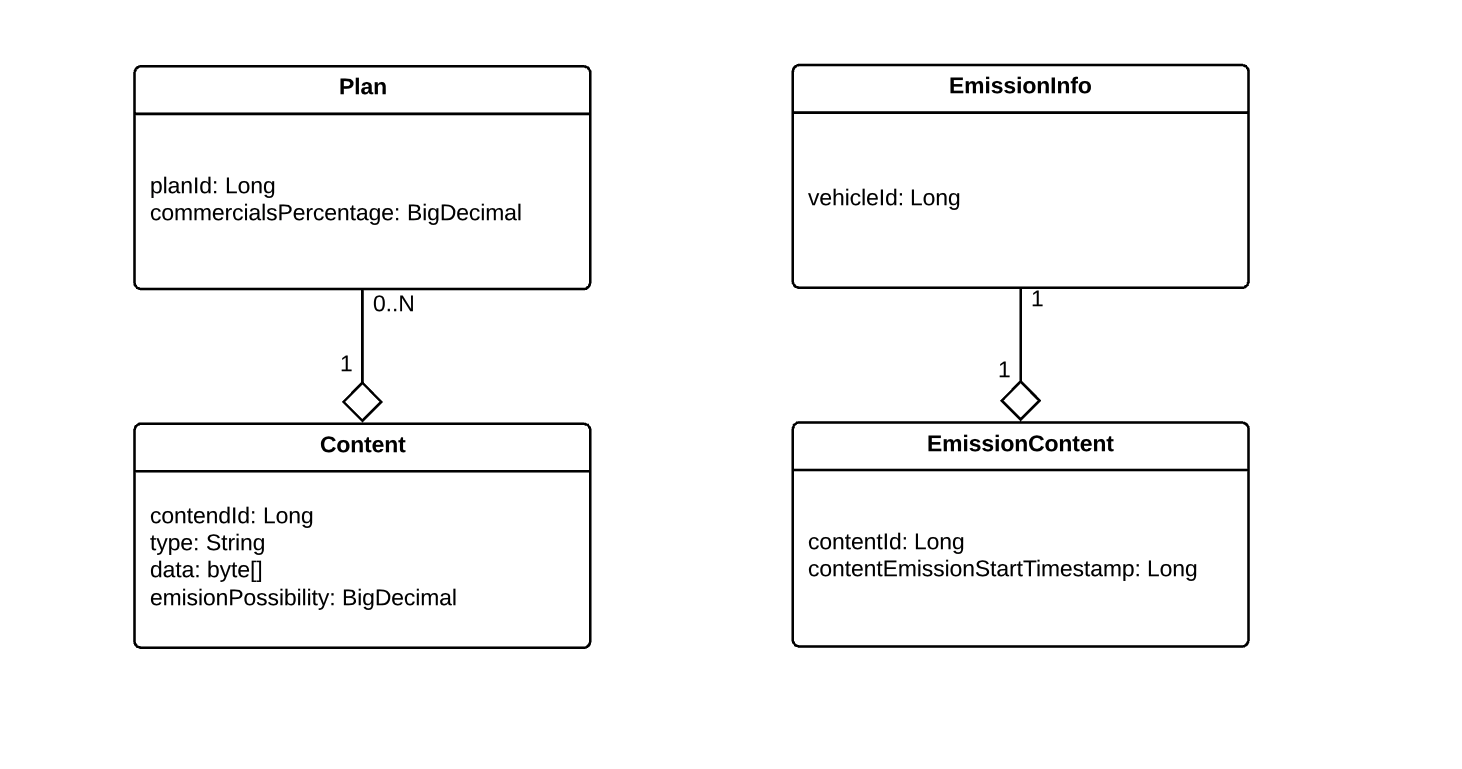
\includegraphics[width=\textwidth]{baza}

     UET przechowuje plan emisji i treści emisji oraz niewysłane komunikaty, które przy ponownym połączeniu mają zostać wysłane.


  \newpage
  \section{Opracuj model, który pozwoli na oszacowanie, z jaką skalą problemu w zakresie transmisji danych mamy tu do czynienia}
    Jeśli treści reklam zostaną załądowane do autobusów przed ich kursem, jedyną komunikacją będzie wtedy jedynie informowanie centrali o wyświetleniach, które są bufforowane jeśli nie ma połączenia. Myślę że nie powinno być problemów z transmisją.


  \newpage
  \section{Zaproponuj harmonogram realizacji tego etapu}
    \subsection{Przygotowania (1 tydzień)}
      - Postawienie środowisk testowych \\
      - Podzielenie zadań na sprinty \\
      - Zebranie informacji potrzebnych do wypełnienia ewidencji (np sprawdzenie możliwości migracji z innej bazy)

    \subsection{Sprinty (12 tygodni)}
      - Utworzenie funkcjonalności oprogramownia \\
      - Otestowanie oprogramowania jednostkowo i integracyjnie

    \subsection{Testy na środowisku testowym (1 tydzień)}
      - Wgranie danych testowych \\
      - Testy end-to-end \\
      - Testy wydajnościowe całego systemu (np gatling)

    \subsection{Migracja na środowisko produkcyjne i testy (1 tydzień)}
      - Wgranie danych produkcyjnych \\
      - Testy end-to-end \\
      - Testy wydajnościowe dla finalnej formy środowiska produkcyjnego

    \subsection{Wdrożenie (1 tydzień)}
      - Wdrożenie początkowo F\&F \\
      - Wdrażanie kontrolując ruch i obciążenie systemu, w razie czego dodanie nowych instancji serwisów


\end{document}